\chapter{INTRODUCTION}
\DeclareGraphicsExtensions{.png,.jpeg,.pdf} 

 \section{Overview}
 Humans have always been curious about the composition of the matter around them. However, the reality is that all entities in the universe are built upon the same foundation - electrons, protons, and neutrons. The protons and neutrons are commonly called nucleons. This leads us to wonder why objects display various properties. Thankfully, a lot of these queries have already been resolved. By comprehending the traits and configurations of these fundamental components, we can understand the formation of atoms, molecules from atoms, and how molecules combine to create matter in our surroundings.

 To understand the properties of matter around us, it's essential to comprehend the nature of its building blocks. One pertinent question is whether these ``building blocks'' are breakable or contain substructures. Unfortunately, these particles are incredibly small, making it difficult to examine them for their properties. The only way to gain insight into their composition is by colliding them with high energy and observing the resulting debris. These experiments, which involve the collision of leptons (spin-1/2 fermions), nucleons (composite structures containing quarks), and heavy ions have provided crucial early information. Many sophisticated experiments are underway, answering several unanswered questions while uncovering new mysteries. 

We currently understand that electrons are fundamental particles. On the other hand, protons and neutrons comprise smaller components called quarks and gluons which bind them together. Quarks are fermions with fractional electromagnetic charge, while gluons are neutral charge (electromagnetic) spin-1 intermediate bosons that act as force carriers between quarks within nucleons by the strong force. Hadrons, which consist of three quarks, are classified as mesons or baryons based on their quark content\footnote{mesons contain a quark and anti-quark pair and baryons contain three quarks.}. The unique properties of nucleons arise from the interactions between quarks and gluons, commonly called partons. Therefore, uncovering the parton structure of nucleons is a critical area of study in high-energy physics. 

There has been a development of theory that successfully explains the bound structure of nucleons. A theory that explains electromagnetic interaction between electromagnetically charged particles via virtual photon exchange is called quantum electrodynamics (QED). The QED, combined with the theory of weak decay of particles via the intermediate vector bosons ($z,\ W^\pm $) by Winberg and Salam, is now commonly called an electroweak theory. The theory of strong interaction, called quantum chromodynamics (QCD), describes the strong interaction between quarks via the exchange of color-charged-gluon.   

After the discovery of the EMC collaboration in 1989, suggesting that the valence quarks contribute little to none to the nucleon's spin, the spin structure of the nucleon remains an unsolved problem thus far, which is widely known as ``proton spin puzzle". 
The unpolarized nucleon structure is known to much higher precision; however, the polarized structure is still not fully understood, specifically the contribution of gluon polarization. It is important to understand how the quarks and gluons dynamics and their spin contribute to the total nucleon property given by the parton distribution functions (PDFs). At the leading twist, three PDFs are enough to describe the nucleon structure: unpolarized (or helicity averaged), helicity PDF, and transversity PDF. Spin asymmetry measurements in polarized  semi-inclusive deep inelastic scattering  (SIDIS) and polarized proton-proton collision ($pp$) have served as crucial tools to understand the (polarized) nucleon structure. The transversity PDF, which is less understood than other PDFs, is lately gaining more attention for its correlation with the tensor charge. This thesis specifically outlines the measurement of two crucial observables, azimuthal correlation asymmetry and the unpolarized cross section, via \dipion channel necessary for the precision measurement of transversity PDF.    

This thesis outline is as follows. In this chapter, I will first provide an overview of elementary particles and a model that describes them. I will also provide the basics of the QCD theory and relevant terminology that will be used frequently hereafter. In the second chapter, I will be more specific about the proton's structure, providing current experimental and theoretical progress, specifically on the transverse momentum-dependent structure of the proton. Chapter 3 will provide experimental aspects; the relativistic heavy ion collider (RHIC) and the solenoidal tracker at RHIC (STAR). Chapters 4  and 5 provide measurement details and results for the  azimuthal correlation asymmetry and unpolarized \dipion cross section. Finally, in Chapter 6, I will summarize the thesis with the relevant outcomes of the measurements. More details, which are not appropriate in the main body of this thesis, will be provided in the appendices. I will refer to the respective appendix whenever relevant in the main body. 

\section{Review of Elementary Particles}

The elementary particle is defined as the fundamental building block of matter, yet this designation is subject to revision as experimental techniques and theoretical frameworks evolve. Whether a particle is elementary or composite is contingent upon the sensitivity of experimental methods and the extent of scientific understanding at a given time. Thus, the characterization of particles as elementary may not be absolute but reflects our current knowledge and technological capability.
 
Initially, the electron, proton, and neutron were considered the fundamental particles, unbreakable without substructures, until the discovery confirmed that the proton is not fundamental: it has something more fundamental structure. As Rutherford's scattering experiment led to the discovery of the atomic nucleus and, eventually, protons and neutrons, the deep inelastic scattering experiment (DIS) led to the discovery of the internal structure of the proton, the quark, as shown in Figure \ref{fig:protonstr}. 
\begin{figure}
    \centering
    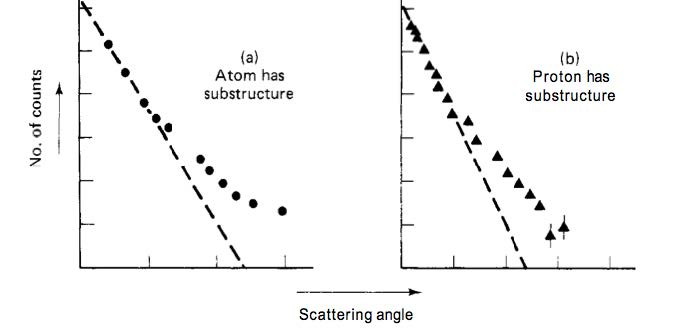
\includegraphics[scale=1.2]{MisImages/martin_halzen_quark.jpg}
    \caption{Left: In Rutherford scattering, the number of particles deflected through large angles indicates that the atom has an internal structure. Right: In deep inelastic scattering, the number of particles scattered through large angles indicates that the proton has an internal structure (quarks). The dashed line represents the expected distribution if the positive charge is uniformly distributed in an atom (left) and proton (right) \cite{HalzenMartin1984}.}
    \label{fig:protonstr}
\end{figure}

Studying the inner workings of a nucleon and its quarks is a complex process that requires advanced detector technologies and particle colliders. These tools allow us to collide particles with enough energy to reveal their inner structure. The wavelength of the probe used in a particle collider is crucial, as it must be smaller than the de-Broglie wavelength\footnote{$\lambda = h/p$, where $h$ = Planck's constant, $p$ = momentum} to probe the nucleon effectively. 

It's worth noting the discovery of elementary particles. Heavier mass particles are produced as the energy of smashing particles increases. Lighter mass particles were discovered first, followed by heavier ones, due to the advancement of particle colliders that achieved higher energy limits.
       
The development of particle discovery started in the 19th century when the modern atomic theory was established. At that time, the exploitable size is $\sim 10^{-10}$m, which is the size of an atom. In 1897, J. J. Thomson discovered an electron and its charge-to-mass ratio by studying the deflection of cathode rays in the external magnetic field \cite{electronJJ}. However, the charge neutrality and large mass of an atom beg speculation that there must be something more massive than an electron and positive in charge that compensates for the electron's charge. This was later confirmed by Rutherford's $\alpha-$scattering experiment \cite{GigerMarsden}, where he passed an $\alpha-$particles\footnote{Helium nucleus consisting of two protons and two neutrons with +2 net charge.} on a gold foil and observed the spectrum of the scattered particles. He observed large deflection in a few of the $\alpha -$particles; however, most remained undisturbed, suggesting that a hard and positive object is in charge at the center and a vast space all around. Rutherford coined the name ``proton" for the nucleus of a hydrogen atom. In 1914, Neils Bhor proposed a model of a hydrogen atom as a negatively charged electron encircling around a positively charged proton at its center. 

There was a problem with Bohr's model, as it failed to explain the atomic structure of higher atomic number elements, for example, a helium atom with two electrons and two protons but four times as massive as hydrogen. It took about two decades until Chadwick discovered the neutron$-$a electrically neutral particle with a mass similar to that of the proton$-$in 1932 \cite{chadwickNeutron}. How positively charged protons reside within the nucleus of size ($\sim 10^{-15}$m) was still puzzling. There should be a stronger force  between nucleons that compensates for the repulsive force and is strong enough to hold protons and neutrons. Yukuwa proposed a theory in 1934 known as the meson theory \cite{Yukawa:1935xg}. He suggested that there should be a force carrier particle, like a photon in electromagnetic interaction, which holds nucleons together, which he called a ``meson". He calculated the mass of the meson to be intermediate between the mass of an electron and a proton. The Yukuwa meson was later discovered as a $\pi-$meson (pion) in 1947. The $\mu-$meson (muon) was also discovered simultaneously with the pion by Powel and co-workers. The muon is the lighter version of an electron and has nothing to do with the strong force.

 Relativistic quantum mechanics started after Dirac's famous relativistic formula,
 \begin{equation}
     E^2 = \vec{p}^2c^2 + m^2 c^4
 \end{equation}
where $E$ is the energy, $\vec{p}$ is the three momentum vector, $m$ is the mass of the particle, and $c$ is the speed of light, the solution of which suggested the existence of antiparticles from the negative energy solution of the relativistic equation, which was not well accepted at that time. However,  the discovery of the positron$-$an positively charged electron$-$ triumphed Dirac's theory in 1931.  Later in 1955 and 1956, antiparticles of proton and neutron, respectively, were discovered.

The discovery of a neutrino follows back to 1930. The missing energy in the nuclear $\beta -$decay kept Pauli skeptical about energy conservation. Fermi proposed that another non-interacting, neutral, and mass-less particle should be emitted along with the electron in the $\beta-$decay. Based on the variation in the energy of the emitted electron considerably, there should not only such particles but two of those are produced. Those particles are named ``neutrinos" by Fermi. 

In late 1947, the neutral kaon ($K^0$) was discovered by Rochester and Butler \cite{Rochester:1947mi} looking at the cloud chamber photograph where it decays to the charge secondaries $\pi^+$ and $\pi^-$. The charged kaon ($K^+$) was discovered in 1949 by Powel. In time, many more particles were found- the $\eta$, the $\phi$, the $\omega$, the $\rho$'s, etc. Heavier particles, $\Lambda$'s, $\Xi$'s, $\Sigma$'s, and $\Delta$'s, were discovered in successive years, which are collectively called strange particles as they produced strangely in the time scale of $\sim 10^{-23}$ seconds and decay relatively slower ($\sim 10^{-10}$ s),  produced by a strong force, and decayed by a weak force. Most of the elementary particles were discovered by the year 1960's making particle physics complete chaos with a swarm of particles. 

To handle this chaos of particles, Murray Gell-Mann proposed a 
``Eightfold Way" of classifying (anti-)particles in 1961 \cite{GellMann:1962}, where he arranged particles in different geometrical patterns (e.g., hexagon to represent meson octet\footnote{eight member family} and a triangular array to represent baryons decuplet\footnote{ten member family}) based on their charge and strangeness. This way of classifying particles led to the discovery of the omega-minus ($\Omega^-$), the missing spot in Gell-Mann's baryon decuplet, and he boldly predicted this particle to exist. The``Eightfold Way" of classifying particles served as a periodic table and initiated the modern era of particle physics.

Later in 1964, the ``Quark Model'' (QM) was proposed by Gell-Mann \cite{GellMann:1964} and independently by Zweig \cite{Zweig:1964}, which suggests that the hadrons\footnote{Baryons and mesons} comprise more fundamental substructures, which Gell-Mann named it ``quarks''. (Anti-)Baryons are composed of three (anti-)quarks, and mesons are composed of a pair of a quark and an antiquark. Quarks come in three flavors; up ($u$), down ($d$), strange ($s$), and three corresponding anti-quarks; anti-up ($\bar{u}$), anti-down($\bar{d}$), and anti-strange ($\bar{s}$). All the quarks have a fractional charge; $u$ has $\frac{2}{3}e$, $d$ and $s$ have $\frac{-1}{3}e$, and their antiparticles have the same magnitude charge, but of opposite sign. Combining these three fundamental quarks, all the baryons and mesons could be reconstructed successfully.  

Besides the intriguing description of the QM, it failed to explain some obvious questions about the fractional charges of (anti-)quarks,  unobserved free (anti-)quarks, and violating the Pauli exclusion principle. Even though the quarks are confined within the hadrons, their existence as a point particle has been observed by the inclusive deep inelastic experiment (DIS), similar to the Rutherford scattering experiment, where most probed particle passes unaffected. In contrast, some are hard-deflected, as shown in figure \ref{fig:protonstr}, which strongly supports the QM. In 1964, O. W. Greenberg suggested the concept of the ``color charge" to the quark to address the QM skepticism. He suggested that each quark, in addition to the fractional electromagnetic charge, has a ``color charge'', which comes in three colors, ``red", ``blue'' and ``green''. A hadron with quarks of different colors (that form a colorless state)is allowed by the exclusion principle. A colorless state is a combination of color and anti-color or a combination of all primary colors in equal proportion. This also explains why quarks are always present within the hadrons and do not exist individually.   

In 1974, the revolutionary $J/\psi$ meson was discovered at Brookhaven National Laboratory (BNL) \cite{E598:1974sol} and Stanford Linear Accelerator (SLAC) \cite{SLAC:1974ind} simultaneously. The $J/\psi$ is a bound state of the charm and anti-charm quarks ($c\bar{c}$)\cite{Clavelli:1974}, which is about three times heavier than the proton and has a much longer lifetime ($10^{20}\ s$). The charm quark was suggested by Borken and Glashow, speculating the parallel between already discovered four types of leptons ($e$,$\mu$, $\nu_{e}$, $\nu_{\mu}$) and only three quarks ($u$, $d$, and $s$). In the successive years, more charmed baryons were discovered (e.g., $\Lambda^+_c (udc)$, $\Sigma_c^+ (uuc)$, $D^0(c\bar{u})$, $D^+(c\bar{d})$), which established the $J/\psi$ as $c\bar{c}$ and again revive the QM. Moreover, the discovery of the ``tau" ($\tau$) in 1975 \cite{Tau:1975} and ``upsilon" ($\Upsilon (b\bar{b})$) in 1977 \cite{Upsilon:1977} adds two leptons (presuming $\nu_{\tau}$) and a ``bottom" or ``beauty" quark. After discovering the ``top'' quark in 1984 \cite{Top:1995}, the quark-lepton symmetry is restored with the six leptons and six quarks. 


\section{Fundamental Forces, Gauge Bosons and The Standard Model}
\subsection{Fundamental Forces and Gauge Bosons}
Four fundamental forces of nature govern the universe's existence: gravity, strong, weak, and electromagnetic forces. All these fundamental forces are discussed in detail in this section. 
\subsubsection{Gravitational Force}
The gravitational force ($F_G$) between two masses varies as an inverse square of their distance ($F_G \sim 1/r^2$). In addition, it is scaled by the masses of objects of interest ($F_G \sim m_1*m_2$). Since this force is more compensated by the concentration of the mass than distance, it's a long-range force. Even though the galaxies are millions of light years apart, they mutually attract each other, maintaining a stable orbit. Albeit gravitational force controls the macroscopic worlds, it is not realizable at the microscopic level. It is negligibly weak at the elementary particle level, which is $\sim 10^{-42}$ times smaller than the electromagnetic force. At the elementary particle level, it becomes significant at the Planck scale ($\sim 10^{-35}$ m), which is extremely small, or at the Planck energy ($\sim 10^{19}$ GeV), which is an extremely high energy, hard to be realizable in real life.       
\subsubsection{Electromagnetic Force}
The nature of electromagnetic force is similar to the gravitational force, except that it is associated with electromagnetically charged particles. It also varies as an inverse square of the distance between the charged particles. It is attractive for the unlike charges and repulsive for the like charges. It is the decisive force that binds electrons and the nucleus to form an atom, atoms together to form molecules, and molecules to form matter that we see in our everyday life. It is also a long-range force, which is $\sim 10^{42}$ times stronger than the gravitational force and a thousand times weaker than the strong force. The charged particles, the electromagnetic field, and their interactions are described by a mathematical framework called Quantum Electrodynamics (QED).   

The gravitational and electromagnetic forces share a common nature: they are long-range forces that vary as an inverse power of distance, $F\sim r^{-n}$. These forces can be felt in everyday life, such as the mutual attraction between the sun and the planets, and the high and low tides on Earth are due to the gravitational. A tiny magnet aligning north-south, the aurora borealis in the polar region, to name a few, are electromagnetic phenomena due to the Earth's magnetic field.  
\subsubsection{Strong Force}
The strong force is about a thousand times stronger than the electromagnetic force, hence the name ``strong force". It is responsible for binding quarks within the nucleon by exchanging a force carrier particle, gluons, and can be felt to a very short distance, a few hadrons in diameter. It behaves as $\sim \exp ^{-r/r_0}/r^2$, where $r_0 \sim 10^{-15}$ m is a hadron diameter and can reach up to $r\leq r_0$. This is the reason why quarks are always confined within the hadrons.   
\subsubsection{Weak Force}
The weak force operates over extremely short distances on the scale of subatomic particles. Its range is governed by the exchange of W and Z bosons, which are the force carriers of the weak force. The range of the weak force is typically on the order of $10^{-18}$ m. The weak force is primarily associated with beta decay, where a neutron can decay into a proton, an electron, and an electron antineutrino. It also involves other particle interactions, including star nuclear fusion reactions.
\subsection{The Standard Model}
The Standard Model (SM) of particle physics is a theoretical framework describing the universe's fundamental particles and forces. It provides a comprehensive understanding of three fundamental forces: the electromagnetic force, the weak nuclear force, and the strong nuclear force. Gravity, the fourth fundamental force, is not included in the Standard Model and is described by a separate theory called general relativity.

SM classifies elementary particles into two categories: quarks and leptons, as shown in figure \ref{fig:sm}. Quarks are the building blocks of protons and neutrons, which make up atomic nuclei. There are six types of quarks: up, down, charm, strange, top, and bottom. Leptons include the electron, muon, and tau particles and their corresponding neutrinos. Each particle has its antiparticle counterpart, with opposite charge and other properties.
\begin{figure}[h]
    \centering
    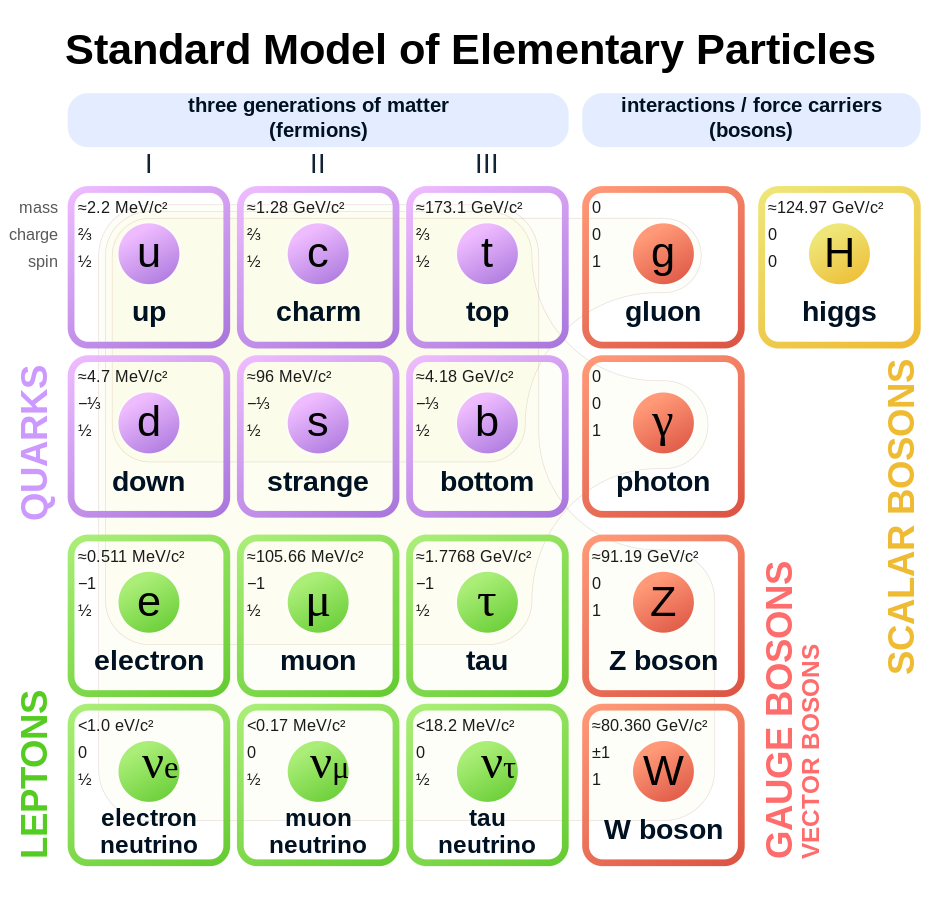
\includegraphics[scale=0.4, trim={0cm 0cm 0cm 2.7cm},clip]{MisImages/Standard_Model_of_Elementary_Particles.svg.png}
    \caption{The standard model of elementary particles \cite{sm}.
    }
    \label{fig:sm}
\end{figure}

The Standard Model describes the fundamental forces as exchanges of particles called gauge bosons. The photon mediates the electromagnetic force, the $W$, and $Z$ bosons mediate the weak nuclear force, and the gluons mediate the strong nuclear force. These gauge bosons carry the forces between particles and govern their interactions.

The Higgs boson is a particle that was discovered in experiments at the Large Hadron Collider (LHC) in 2012 \cite{ATLAShiggs:2012, CMShiggs:2012}. It is associated with the Higgs field, which permeates all of space. The Higgs field gives mass to other particles through their interactions with it. The discovery of the Higgs boson confirmed the mechanism responsible for particle mass in the Standard Model.

\section{Strong Interaction and Quantum Chromodynamics}
Quantum chromodynamics (QCD) is a gauge field theory that describes the strong interactions of colored quarks and gluons in the SU(3) component of the SU(3)$\times$ SU(2)$\times$ SU(1) standard model of particle physics. The QCD lagrangian is given by \cite{Workman:2022}
    \begin{equation}
        \mathcal{L} = \sum_q \bar{\psi}_{q,a}(i\gamma^\mu \partial_\mu \delta_{ab} - g_s \gamma^\mu t^C_{ab} \mathcal{A}^C_\mu - m_q \delta_{ab})\psi_{q,b}-\frac{1}{4}F^A_{\mu\nu}F^{A \mu \nu},
    \end{equation}
where repeated indices are summed over. The $\gamma^\mu$ are Dirac $\gamma-$matrices. The $\psi_{q,a}$ are quark field spinors for a quark flavor $ q$ and mass $m_q$, with color index $a$. The color index $a$ runs from 1 to 3, corresponding to the number of color charges in the QCD ($N_c = 3$). The gluon field is represented by $\mathcal{A}^C$, where $C$ runs from 1 to 8 representing eight types of gluons, which transform under the adjoint representation of the SU(3) color group. The $t_{ab}^C$ are the generators of the SU(3) group in the form of eight 3$\times$3 matrices, which encodes the fact that gluon's interaction with the quark rotates the quark's color in SU(3) space. The $g_s(= \frac{\alpha_s^2}{4\pi})$ is a QCD coupling constant, which is the fundamental parameter of the QCD. The $F_{\mu\nu}^A$ is a field tensor given by 
   \begin{equation}
       F_{\mu\nu}^A = \partial_\mu \mathcal{A}^A_\nu - \partial_\nu \mathcal{A}_\mu^A - g_s f_{ABC}\mathcal{A}_\mu^B\mathcal{A}_\nu^C, 
       \end{equation}
with $[t^A,t^B]= if_{ABC}t^C$, where $f_{ABC}$ are the structure constants of the SU(3) group. 

The QCD theory applies when the strong coupling constant $\alpha_s$ is small, at which quarks are essentially ``free'' within the nucleon. This regime corresponds to the very high energy limit (or a very short distance), where QCD perturbation theory successfully describes the strong interaction between partons. However, the self-gluon  interaction makes the $g_s$ to be varied with the scale of the process, which causes $g_s$ to be small in the short distance (high energy) and large in the longer distance (small distance), leading to the phenomena called ``asymptotic freedom". At the leading order, the strong coupling constant $\alpha_s$ can be expressed as \cite{Surrow:2017}
\begin{equation}
    \alpha_s(Q^2) = \frac{4\pi}{(11-2n_f/3)ln(\frac{Q^2}{\Lambda^2})},
\end{equation}
where $n_f$ is the number of quark flavors and $\Lambda$ is a free scale parameter. The logarithmic dependence of the $\alpha_s$ is because the anti-screening of the effective color charge is because of the gluon bubbles, as shown in figure \ref{fig:glueball}. In any cases when $(11-2n_f/3)>0$, the anti-screening due to the gluon self-interaction dominates, and as a consequence, the $\alpha_s$ decrease with increasing $Q^2$ and becomes relatively weak at the shorter distances. The experimental measurement of $\alpha_s(Q^2)$ as a function of $Q$ from the world data is shown in figure \ref{fig:alphasvsQ}.
\begin{figure}
    \centering
    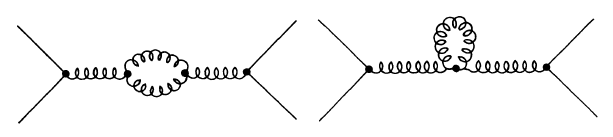
\includegraphics[scale=0.5]{MisImages/glueballs.png}
    \caption{Gluon self-interactions responsible for the anti-screening of the color charge.}
    \label{fig:glueball}
\end{figure}
\begin{figure}[h]
    \centering
    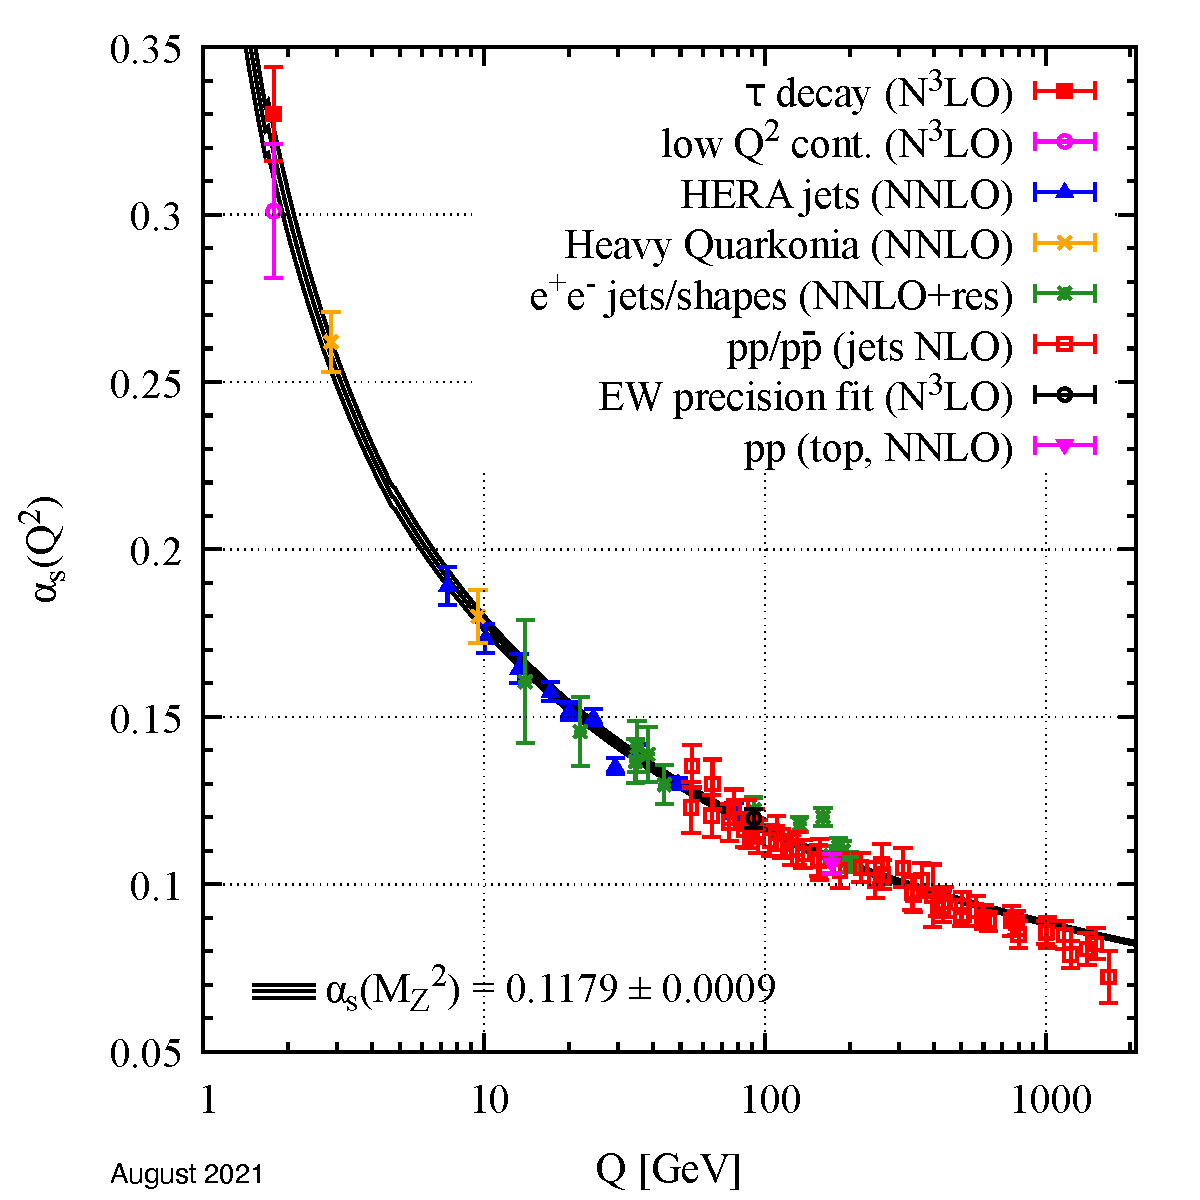
\includegraphics[scale=0.65]{MisImages/alphasVsQ2021.pdf}
    \caption{ The running coupling constant from the experiments as a function of the energy scale Q \cite{alphasVsQ:2022}.}
    \label{fig:alphasvsQ}
\end{figure}

When the $Q^2$ is small (at longer distances), the coupling becomes strong that the perturbative theory is no longer applicable; this region corresponds to the non-perturbative regime. The self-interaction of gluons forms the ``glue tube'' by squeezing the lines of forces together, which implies the quark-antiquark potential of the form $V(r)=-\frac{4}{3}\frac{\alpha_s}{r} + \lambda r$. Because of this linear potential, it requires infinite energy to separate quark and antiquark pair, resulting in the phenomenon called ``confinement". The ``confinement'' suggests that quarks and gluons are confined within the nucleons.   

    


 